% Source: Code/ML_overlay/ir_rgb_registration/paper/figures/fig_affine_raft_architecture.tex
% Experiment 3: Affine + Dense Residual RAFT Architecture
% J.C. Vaught
\documentclass[tikz,border=8pt]{standalone}

\usepackage[T1]{fontenc}
\usepackage{lmodern}
\usepackage{amsmath,amssymb}

\usetikzlibrary{arrows.meta,positioning,calc,fit,decorations.pathreplacing,backgrounds}

% ── Brand colours ──────────────────────────────────────────────────
\definecolor{Garnet}{HTML}{73000A}
\definecolor{Rose}{HTML}{CC2E40}
\definecolor{Atlantic}{HTML}{466A9F}
\definecolor{Congaree}{HTML}{1F414D}
\definecolor{Horseshoe}{HTML}{65780B}
\definecolor{Honeycomb}{HTML}{A49137}
\definecolor{Black90}{HTML}{363636}
\definecolor{Black70}{HTML}{5C5C5C}
\definecolor{Black50}{HTML}{A2A2A2}
\definecolor{Black30}{HTML}{C7C7C7}
\definecolor{Black10}{HTML}{ECECEC}

\tikzset{
  every node/.style={font=\sffamily\small},
  block/.style={
    draw=#1, fill=#1!8, line width=0.9pt,
    minimum height=0.85cm, minimum width=1.6cm,
    inner sep=4pt, align=center,
    font=\sffamily\footnotesize},
  block/.default={Black90},
  tensor/.style={
    font=\sffamily\scriptsize, text=Black70, align=center},
  arr/.style={-{Stealth[length=2.6pt,width=2.4pt]},
              line width=0.7pt, color=#1},
  arr/.default={Black90},
  sumnode/.style={
    draw=Horseshoe, fill=Horseshoe!12, line width=0.9pt,
    circle, minimum size=0.6cm,
    inner sep=0pt, font=\sffamily\normalsize},
  groupbox/.style={
    draw=#1, line width=1.1pt, dashed, dash pattern=on 4pt off 2.5pt,
    fill=#1!4, inner sep=8pt},
  annot/.style={font=\sffamily\tiny, text=Black70},
}

\begin{document}
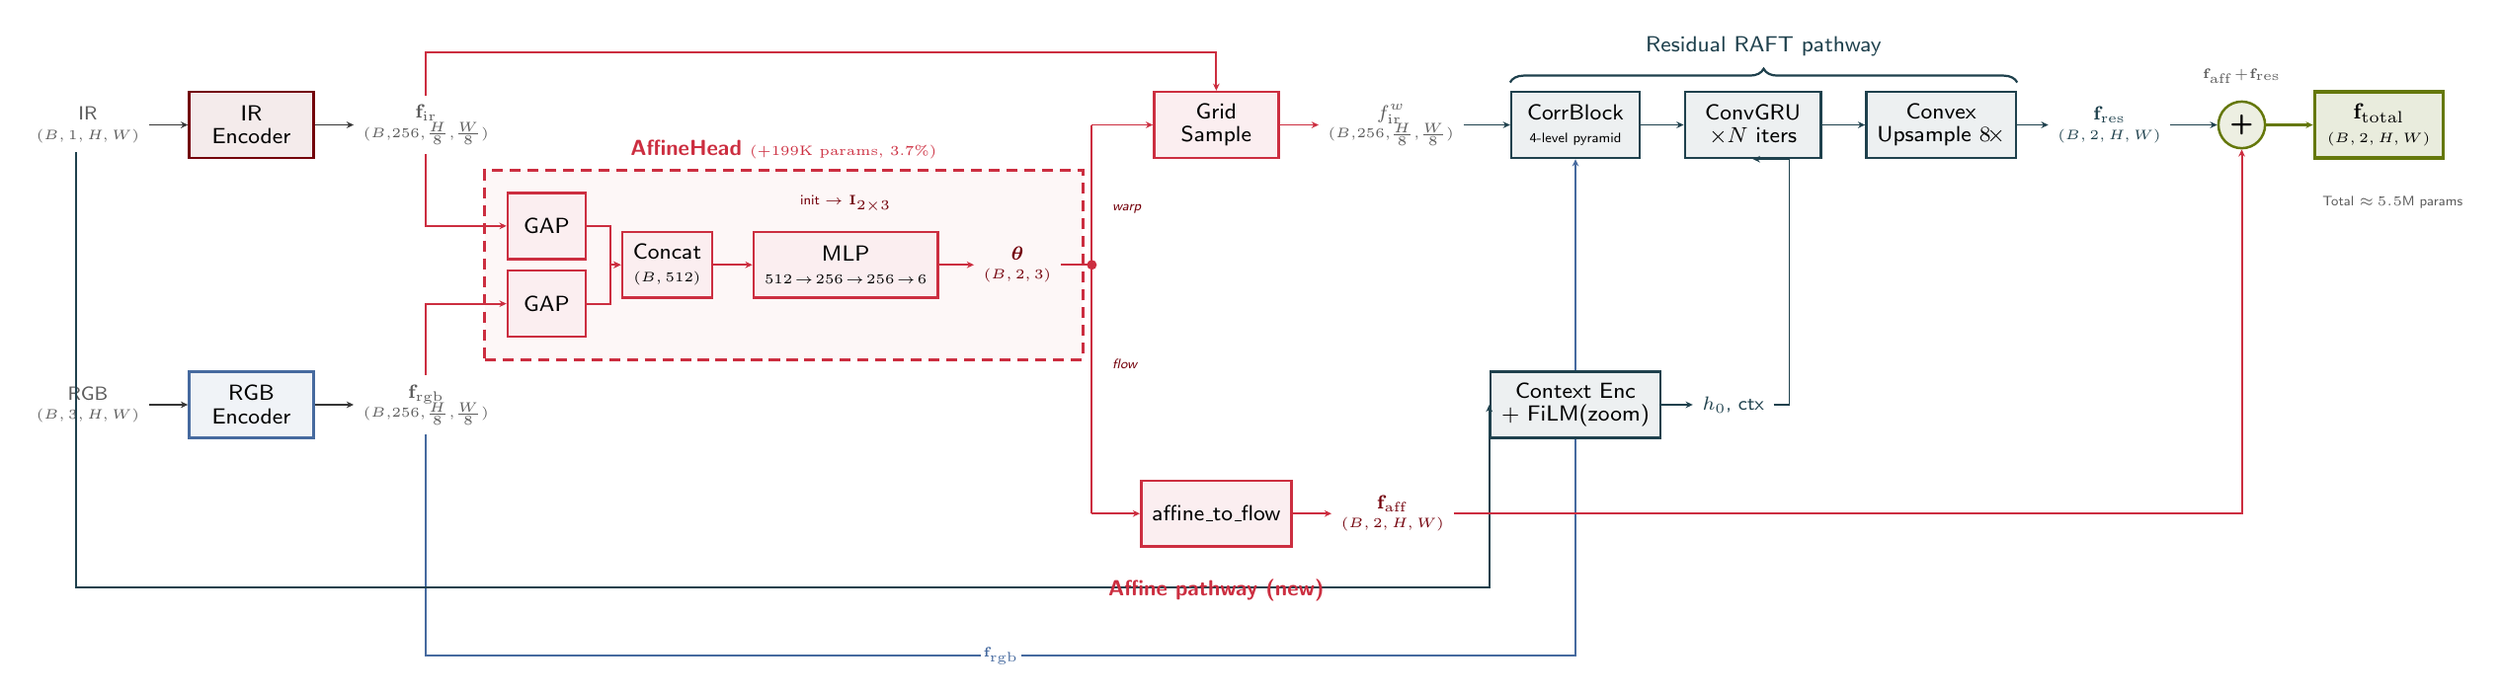
\begin{tikzpicture}[node distance=0.6cm and 0.5cm]

% =====================================================================
%   Row A (y=0):     IR Enc -> fmap_ir ... Grid Sample -> fmap_ir_w
%                    -> CorrBlock -> ConvGRU -> Upsample -> F_res -> (+) -> F_total
%   Row M (y=-1.8):  [AffineHead] GAP+GAP -> Concat -> MLP -> theta
%   Row B (y=-3.6):  RGB Enc -> fmap_rgb
%   Row F (y=-5.0):  affine_to_flow -> F_aff | Context Enc -> h0,ctx
%   Row G (y=-6.2):  fmap_rgb routing (under everything) and F_aff to (+)
% =====================================================================

% ── Row A: IR ────────────────────────────────────────────────────
\node[tensor] (ir_in) at (0,0) {IR\\[-1pt]{\tiny$(B,1,H,W)$}};
\node[block=Garnet, right=0.5cm of ir_in] (ir_enc) {IR\\[-1pt]Encoder};
\node[tensor, right=0.5cm of ir_enc] (fmap_ir)
  {$\mathbf{f}_{\mathrm{ir}}$\\[-1pt]{\tiny$(B,\!256,\!\tfrac{H}{8},\!\tfrac{W}{8})$}};
\draw[arr] (ir_in) -- (ir_enc);
\draw[arr] (ir_enc) -- (fmap_ir);

% ── Row B: RGB ───────────────────────────────────────────────────
\node[tensor] (rgb_in) at (0,-3.6) {RGB\\[-1pt]{\tiny$(B,3,H,W)$}};
\node[block=Atlantic, right=0.5cm of rgb_in] (rgb_enc) {RGB\\[-1pt]Encoder};
\node[tensor, right=0.5cm of rgb_enc] (fmap_rgb)
  {$\mathbf{f}_{\mathrm{rgb}}$\\[-1pt]{\tiny$(B,\!256,\!\tfrac{H}{8},\!\tfrac{W}{8})$}};
\draw[arr] (rgb_in) -- (rgb_enc);
\draw[arr] (rgb_enc) -- (fmap_rgb);

% =====================================================================
% AffineHead -- Row M
% =====================================================================

% GAP blocks
\node[block=Rose, minimum width=1.0cm]
  at ($(fmap_ir) + (1.55,-1.3)$) (gap_ir) {GAP};
\node[block=Rose, minimum width=1.0cm]
  at ($(gap_ir) + (0,-1.0)$) (gap_rgb) {GAP};

% Feature maps -> GAPs
\draw[arr=Rose] (fmap_ir.south) |- (gap_ir.west);
\draw[arr=Rose] (fmap_rgb.north) |- (gap_rgb.west);

% Concat
\node[block=Rose, minimum width=1.15cm]
  at ($(gap_ir)!0.5!(gap_rgb) + (1.55,0)$) (concat)
  {Concat\\[-1pt]{\tiny$(B,512)$}};
\draw[arr=Rose] (gap_ir.east) -- ++(0.3,0) |- (concat.west);
\draw[arr=Rose] (gap_rgb.east) -- ++(0.3,0) |- (concat.west);

% MLP
\node[block=Rose, right=0.5cm of concat, minimum width=2.1cm] (mlp)
  {MLP\\[-1pt]{\tiny$512\!\to\!256\!\to\!256\!\to\!6$}};
\draw[arr=Rose] (concat) -- (mlp);

% Identity-init annotation
\node[annot, above=0.12cm of mlp, text=Garnet]
  {init $\to \mathbf{I}_{2\times3}$};

% Theta
\node[tensor, right=0.45cm of mlp, text=Garnet] (theta)
  {$\boldsymbol{\theta}$\\[-1pt]{\tiny$(B,2,3)$}};
\draw[arr=Rose] (mlp) -- (theta);

% Dashed AffineHead box
\begin{scope}[on background layer]
  \node[groupbox=Rose,
        fit=(gap_ir)(gap_rgb)(concat)(mlp)(theta),
        label={[font=\sffamily\footnotesize\bfseries,
                text=Rose]above:%
          AffineHead {\normalfont\tiny(+199K params, 3.7\%)}}]
    (affinebox) {};
\end{scope}

% =====================================================================
% Theta fan-out via vertical bus
% =====================================================================
\coordinate (tfork) at ([xshift=0.4cm]theta.east);
\draw[Rose, line width=0.7pt] (theta.east) -- (tfork);
\fill[Rose] (tfork) circle (1.8pt);

% Vertical bus endpoints
\coordinate (tfork_up) at ($(tfork) + (0,1.8)$);
\coordinate (tfork_dn) at ($(tfork) + (0,-3.2)$);
\draw[Rose, line width=0.7pt] (tfork_up) -- (tfork_dn);

% ── Use 1: theta -> Grid Sample (Row A) ─────────────────────────
\node[block=Rose, minimum height=0.85cm]
  at ($(tfork_up) + (1.6,0)$) (warp)
  {Grid\\[-1pt]Sample};
\draw[arr=Rose] (tfork_up) -- (warp.west);

% fmap_ir across top to Grid Sample
\draw[arr=Rose]
  (fmap_ir.north) -- ++(0,0.55) -| (warp.north);

% Warped features output
\node[tensor, right=0.5cm of warp] (fmap_ir_w)
  {$f_{\mathrm{ir}}^{w}$\\[-1pt]{\tiny$(B,\!256,\!\tfrac{H}{8},\!\tfrac{W}{8})$}};
\draw[arr=Rose] (warp) -- (fmap_ir_w);

% ── Use 2: theta -> affine_to_flow (Row F) ──────────────────────
\node[block=Rose, minimum width=1.65cm]
  at ($(tfork_dn) + (1.6,0)$) (a2f)
  {affine\_to\_flow};
\draw[arr=Rose] (tfork_dn) -- (a2f.west);

% F_aff output rightward
\node[tensor, right=0.5cm of a2f, text=Garnet] (aflow)
  {$\mathbf{f}_{\mathrm{aff}}$\\[-1pt]{\tiny$(B,2,H,W)$}};
\draw[arr=Rose] (a2f) -- (aflow);

% Labels on theta bus (right side)
\node[annot, text=Garnet, anchor=west]
  at ([xshift=4pt]$(tfork)!0.4!(tfork_up)$)
  {\textit{warp}};
\node[annot, text=Garnet, anchor=west]
  at ([xshift=4pt]$(tfork)!0.4!(tfork_dn)$)
  {\textit{flow}};

% =====================================================================
% CorrBlock -- Row A
% =====================================================================
\node[block=Congaree, right=0.6cm of fmap_ir_w, minimum width=1.65cm] (corr)
  {CorrBlock\\[-1pt]{\tiny 4-level pyramid}};
\draw[arr=Congaree] (fmap_ir_w) -- (corr);

% fmap_rgb to CorrBlock: route UNDER entire diagram to avoid crossing
% the AffineHead box. Go south from fmap_rgb, then east at y=-6.2,
% then north up to CorrBlock.south.
\draw[arr=Atlantic, line width=0.7pt]
  (fmap_rgb.south) -- ++(0,-2.85) -| (corr.south);

% Label on the fmap_rgb horizontal routing segment
\coordinate (rgb_bot_left) at ([yshift=-2.85cm]fmap_rgb.south);
\coordinate (rgb_bot_right) at (rgb_bot_left -| corr.south);
\node[annot, text=Atlantic, fill=white, inner sep=1pt]
  at ($(rgb_bot_left)!0.5!(rgb_bot_right)$)
  {$\mathbf{f}_{\mathrm{rgb}}$};

% =====================================================================
% Context Encoder -- Row F (right side, same y as affine_to_flow)
% =====================================================================
\node[block=Congaree, minimum width=1.65cm]
  at ($(corr) + (0, -3.6)$) (ctx)
  {Context Enc\\[-1pt]+ FiLM(zoom)};

% IR input to Context Encoder: route along left margin
\draw[arr=Congaree]
  ([xshift=-0.15cm]ir_in.south) -- ++(0,-5.6) -| (ctx.west);

% h0, ctx output
\node[tensor, right=0.4cm of ctx, text=Congaree] (hctx) {$h_0$, ctx};
\draw[arr=Congaree] (ctx) -- (hctx);

% =====================================================================
% ConvGRU -- Row A
% =====================================================================
\node[block=Congaree, right=0.55cm of corr, minimum width=1.75cm] (gru)
  {ConvGRU\\[-1pt]$\times N$ iters};
\draw[arr=Congaree] (corr) -- (gru);

% Context feeds into GRU from below
\draw[arr=Congaree]
  (hctx.east) -- ++(0.2,0) |- (gru.south);

% =====================================================================
% Convex Upsample -- Row A
% =====================================================================
\node[block=Congaree, right=0.55cm of gru, minimum width=1.55cm] (upsample)
  {Convex\\[-1pt]Upsample $8\!\times$};
\draw[arr=Congaree] (gru) -- (upsample);

% Residual flow
\node[tensor, right=0.4cm of upsample, text=Congaree] (rflow)
  {$\mathbf{f}_{\mathrm{res}}$\\[-1pt]{\tiny$(B,2,H,W)$}};
\draw[arr=Congaree] (upsample) -- (rflow);

% =====================================================================
% Summation -- Row A
% =====================================================================
\node[sumnode, right=0.6cm of rflow] (plus) {\textbf{+}};
\draw[arr=Congaree] (rflow) -- (plus);

% F_aff routes right along Row F then up to summation
\draw[arr=Rose, line width=0.7pt]
  (aflow.east) -| (plus.south);

% =====================================================================
% Final output -- Row A
% =====================================================================
\node[block=Horseshoe, right=0.6cm of plus, minimum width=1.65cm,
      line width=1.2pt, fill=Horseshoe!14] (total)
  {$\mathbf{f}_{\mathrm{total}}$\\[-1pt]{\tiny$(B,2,H,W)$}};
\draw[arr=Horseshoe, line width=0.9pt] (plus) -- (total);

% =====================================================================
% ANNOTATIONS
% =====================================================================

% Summation formula
\node[annot, above=0.1cm of plus]
  {$\mathbf{f}_{\mathrm{aff}} \!+\! \mathbf{f}_{\mathrm{res}}$};

% Parameter count
\node[annot, anchor=north west, text=Black70]
  at ([yshift=-0.35cm]total.south west)
  {Total ${\approx}\,5.5$M params};

% Residual RAFT pathway brace
\draw[decorate,decoration={brace,amplitude=5pt,raise=3pt},
      Congaree, line width=0.8pt]
  (corr.north west) -- (upsample.north east)
  node[midway, above=9pt, font=\sffamily\footnotesize, text=Congaree]
    {Residual RAFT pathway};

% Affine pathway label
\node[font=\sffamily\footnotesize\bfseries, text=Rose]
  at ($(a2f.south) + (0,-0.55)$)
  {Affine pathway (new)};

\end{tikzpicture}
\end{document}
